% Chapter 3

\chapter{Classifier Features and Logical Schema} % Main chapter title

\label{Chapter3} % For referencing the chapter elsewhere, use \ref{Chapter3} 

\lhead{Chapter 3. \emph{Classifier Features}} % This is for the header on each page - perhaps a shortened title

%----------------------------------------------------------------------------------------

\section{Introduction}
In the previous chapter, a background about text and email classification was presented. Also, technologies that are related to text classification were introduced. Some related applications that are similar to Smart Email with their features were discussed.

In this chapter, the logical schema for the smart email classifier is discussed. In section 3.2, the features used for email classification is presented. Section 3.3 includes the detailed classifier features. In section 3.4, the Data Model (DM) and Entity Relationship Model (ERD) are presented. Section 3.5 presents the tuple of classifier features used as an input for the email classifier.
%==============================================================================
\newpage
\section {Classifier Features}
\begin{longtable}{|>{\centering}p{2.5cm}|>{\centering}p{3cm}|>{\centering}p{3cm}|>{\centering}p{3cm}|}
\hline
\multirow{19}{2.5cm}{Features needed for the email classifier (Automatic Categorization
of emails into folders)}
 & \multicolumn{3}{c|}{Features}\tabularnewline
\cline{2-4}
\cline{2-4} 
 & Email & Receiver & Attachment\tabularnewline
\cline{2-4} 
 & Email ID \cite{Anatomy00} & Domain of receiver \cite{Carmona2011} \cite{MANUEL11} &  Attachment  type \cite{Carmona2011} \cite{MANUEL11}\tabularnewline
\cline{2-4} 
 & Body Length \cite{Carmona2011} \cite{MANUEL11} & Number of CC \cite{Carmona2011} \cite{MANUEL11} & Has an attachment \cite{Carmona2011} \cite{MANUEL11}\tabularnewline
\cline{2-4} 
 & Content Type \cite{Anatomy00} & Number of receivers \cite{Carmona2011} \cite{MANUEL11} & Number of attachments \cite{Carmona2011} \cite{MANUEL11}\tabularnewline
\cline{2-4} 
 & Domain of sender \cite{Carmona2011} \cite{MANUEL11} & Number of To \cite{Carmona2011} \cite{MANUEL11} & \tabularnewline
\cline{2-4} 
 & Email Date \cite{KIRI2004} \cite{Anatomy00} & Receiver Username \cite{Carmona2011} \cite{MANUEL11} & \tabularnewline
\cline{2-4} 
 & Email Sender \cite{Carmona2011} \cite{RON04} \cite{Anatomy00} \cite{MANUEL11} &  & \tabularnewline
\cline{2-4} 
 & Email Signature \cite{MANUEL11} &  & \tabularnewline
\cline{2-4} 
 & Email Subject \cite{Carmona2011} \cite{RON04} \cite{MANUEL11} &  & \tabularnewline
\cline{2-4} 
 & Is Bcc \cite{Carmona2011} \cite{RON04} \cite{MANUEL11} &  & \tabularnewline
\cline{2-4} 
 & Is distribution List \cite{Carmona2011} \cite{MANUEL11} &  & \tabularnewline
\cline{2-4} 
 & Language \cite{Carmona2011} \cite{MANUEL11} &  & \tabularnewline
\cline{2-4} 
 & MIME Version \cite{Anatomy00} &  & \tabularnewline
\cline{2-4} 
 & Number of punctuation Letters \cite{Carmona2011} \cite{MANUEL11} &  & \tabularnewline
\cline{2-4} 
 & Percentage of capital letters \cite{Carmona2011} \cite{MANUEL11} &  & \tabularnewline
\cline{2-4} 
 & Sender Username \cite{Carmona2011} \cite{MANUEL11} &  & \tabularnewline
\cline{2-4} 
 & Subject Length \cite{Carmona2011} \cite{MANUEL11} &  & \tabularnewline
\cline{2-4} 
 & Wordgram Frequency \cite{Carmona2011} \cite{RON04} \cite{MANUEL11} &  & \tabularnewline
\hline
\end{longtable}
%----------------------------------------------------------------------
\section {Detailed Classifier Features}

\begin{longtable}{|>{\centering}p{2cm}|>{\centering}p{2.5cm}|>{\centering}p{3cm}|>{\centering}p{3cm}|>{\centering}p{3cm}|}
\hline 
Category & Feature & Description & Values & Source (preparation)\tabularnewline
\hline
\hline 
Email & Email ID \cite{Anatomy00} & Identifier for the email message & Long & System maintained primary key\tabularnewline
\hline 
 & Domain of sender \cite{Carmona2011} \cite{MANUEL11} & Mail Service Provider (gmail.com, hotmail.com, ..etc) & String & Obtained from the sender's email, by taking the substring after the
'@' character\tabularnewline
\hline 
 & Language \cite{Carmona2011} \cite{MANUEL11} & Dominant language in the email body & String & Use a special module to detect the language type of the email body\tabularnewline
\hline 
 & Email Sender \cite{Carmona2011} \cite{RON04} \cite{Anatomy00} \cite{MANUEL11} & Email address of the sender & String & Obtained directly from the email header\tabularnewline
\hline 
 & Content Type \cite{Anatomy00} & Content type  & String & Obtained directly from the email header\tabularnewline
\hline 
 & Email Date \cite{KIRI2004} \cite{Anatomy00} & Date of sending the email represented as the number of milliseconds
since January 1, 1970, 00:00:00 GMT & Long & The date is obtained directly from the email header and then transformed
to the long representation\tabularnewline
\hline 
 & MIME Version \cite{Anatomy00} & MIME is an internet standard to extend the format of the email to
support non-ASCII data & Integer & Obtained directly from the email header\tabularnewline
\hline 
 & Bcc \cite{Carmona2011} \cite{RON04} \cite{MANUEL11} & List of email receivers as Bcc & Each recipient is represented as a boolean attribute in the feature
tuple. & Obtained directly from the email header \tabularnewline
\hline 
 & Number of punctuation Letters \cite{Carmona2011} \cite{MANUEL11} & Number of punctuation characters in the body & Integer & Count the number of punctuation letters in the email body\tabularnewline
\hline 
 & Is distribution List \cite{Carmona2011} \cite{MANUEL11} & Flag to indicate whether the client received this email from a group/distribution
list or not & Boolean & Obtained directly from email header\tabularnewline
\hline 
 & Email Signature \cite{MANUEL11} & Signature of the email sender, at the end of the email & String & The signature is extracted from email body\tabularnewline
\hline 
 & Wordgram Frequency \cite{Carmona2011} \cite{RON04} \cite{MANUEL11} & Email Wordgram Frequency & Integer & Count the number of wordgrams in the email\tabularnewline
\hline 
 & Subject Length \cite{Carmona2011} \cite{MANUEL11} & Length of the email subject & Integer & Calculate the size of the subject string\tabularnewline
\hline 
 & Percentage of capital letters \cite{Carmona2011} \cite{MANUEL11} & Percentage of the capital letters to the letters in the email body & Double & Count the number of capital letters and divide it by the sum of the
sizes of all ASCII words in the email body\tabularnewline
\hline 
 & Body Length \cite{Carmona2011} \cite{MANUEL11} & Size of the email body & Integer & Calculate the size of the body string\tabularnewline
\hline 
 & Sender Username \cite{Carmona2011} \cite{MANUEL11} & Name of Sender & String & Obtained directly from email header\tabularnewline
\hline 
 & Total Number of words & Number of words in the email body & Integer & Calculate the number of words in the email body\tabularnewline
\hline 
 & Email Subject \cite{Carmona2011} \cite{RON04} \cite{MANUEL11} & Subject of the email & String & Obtained directly from the email header\tabularnewline
\hline 
Receiver & Receiver Username \cite{Carmona2011} \cite{MANUEL11} & Name of receiver & String & Obtained directly from email header\tabularnewline
\hline 
 & Number of receivers \cite{Carmona2011} \cite{MANUEL11} & Number of email receivers & Integer & Count the number of receivers obtained from email header\tabularnewline
\hline 
 & Number of CC \cite{Carmona2011} \cite{MANUEL11} & Number of CC recipients & Integer & Count the number of CC recipients obtained from email header\tabularnewline
\hline 
 & Number of To \cite{Carmona2011} \cite{MANUEL11} & Number of CC & Integer & Count the number of receivers mentioned in the TO header\tabularnewline
\hline 
 & Domain of receiver \cite{Carmona2011} \cite{MANUEL11} & Mail Service Provider(s) for the receiver(s) & String & Obtained directly from email header\tabularnewline
\hline 
Attachment & Number of attachments \cite{Carmona2011} \cite{MANUEL11} & Number of attached files in the email  & Integer & Count the number of attachments obtained from the IMAP interface\tabularnewline
\hline 
 &  Attachment  type \cite{Carmona2011} \cite{MANUEL11} & Type of attachment & String & 	Has an attachment \cite{Carmona2011} \cite{MANUEL11}	Flag to denote whether the email
has an attachment	Boolean 	If the number of attachment is zero, return
false, else return true
\tabularnewline
\hline
\end{longtable}
%----------------------------------------------------------------------
\newpage
\section{Logical Schema for Classifiers Features: Data Model – ERD and ETS}
Figure 3.1 illustrates the logical conceptual view of the classifier features Data Model (DM) and Figure 3.2 illustrates the mapping of DM into Entity Relationship Diagram (ERD).
\begin{figure}
  \centering
  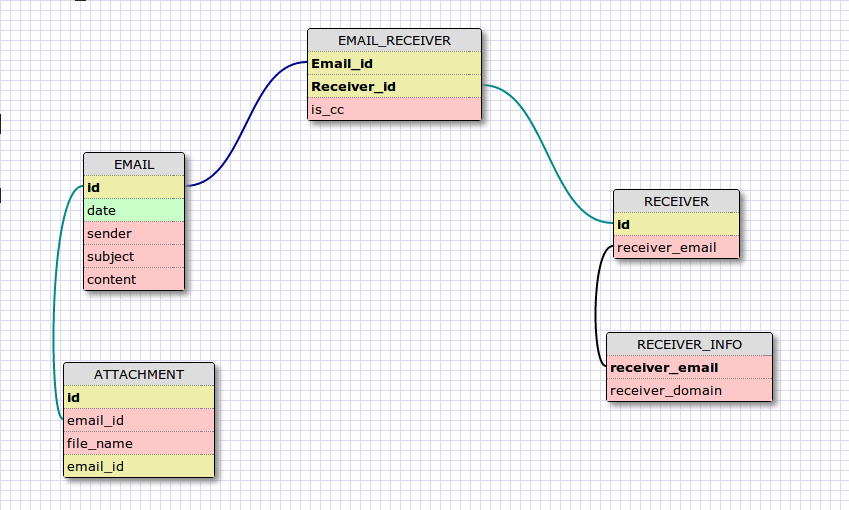
\includegraphics[scale=0.5] {erd1.png}
  \caption[Logical Conceptual View of the classifier features Data Model (DM)] {Logical Conceptual View of the classifier features Data Model (DM)}
\end{figure}

\begin{figure}
  \centering
  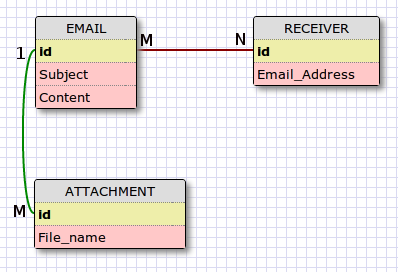
\includegraphics[scale=0.7]{erd2.png}
  \caption[Mapping DM into Entity Relationship Diagram (ERD)] {Mapping DM into Entity Relationship Diagram (ERD)}
\end{figure}


\begin{tabular}{|>{\centering}p{3cm}|>{\centering}p{3cm}|>{\centering}p{2.5cm}|>{\centering}p{3cm}|}
\hline 
\textbf{Project}: \underbar{Smart Email } & \textbf{Subject}: \underbar{Classifier Features} & \multicolumn{2}{>{\centering}p{5.5cm}|}{\textbf{Page}: 1/1}\tabularnewline
\hline
\hline 
\textbf{Entity}: \underbar{Email}  & \textbf{Date}: \underbar{Thursday,}

\underbar{March 1,2012} & \multicolumn{2}{>{\centering}p{5.5cm}|}{\textbf{Analyst}:}\tabularnewline
\hline 
\textbf{Attribute } & \textbf{Type} & \textbf{Size} & \textbf{Validation / desc}\tabularnewline
\hline 
Id  & Integer & 4 Bytes & Primary Key, system maintained,used to identify emails\tabularnewline
\hline 
date & Date & - & the date the email was received in\tabularnewline
\hline 
sender & String & 40 Characters & The email address of the email sender\tabularnewline
\hline 
subject & String & 40 Characters & The Subject of the email\tabularnewline
\hline 
content & Text & - & The body of the email\tabularnewline
\hline
\end{tabular}

\newpage

\begin{tabular}{|>{\centering}p{3cm}|>{\centering}p{3cm}|>{\centering}p{2.5cm}|>{\centering}p{3cm}|}
\hline 
\textbf{Project}: \underbar{Smart Email} & \textbf{Subject}: \underbar{Classifier Features} & \multicolumn{2}{>{\centering}p{5.5cm}|}{\textbf{Page}: 1/1}\tabularnewline
\hline
\hline 
\textbf{Entity}: \underbar{ATTACHMENT} & \textbf{Date}: \underbar{Thursday,}

\underbar{March 1, 2012} & \multicolumn{2}{>{\centering}p{5.5cm}|}{\textbf{Analyst}:}\tabularnewline
\hline 
\textbf{Attribute} & \textbf{Type} & \textbf{Size} & \textbf{Validation / desc}\tabularnewline
\hline 
Id & Integer & 4 Bytes & Primary Key, system maintained, used to identify different attachments\tabularnewline
\hline 
email\_id & Integer & 4 Bytes & Foreign key to EMAIL.id\tabularnewline
\hline 
file\_name & String & 40 Characters & Name of the attachment\tabularnewline
\hline
\end{tabular}

\newpage

\begin{tabular}{|>{\centering}p{3cm}|>{\centering}p{3cm}|>{\centering}p{2.5cm}|>{\centering}p{3cm}|}
\hline 
\textbf{Project}: \underbar{Smart Email} & \textbf{Subject}: \underbar{Classifier Features} & \multicolumn{2}{>{\centering}p{5.5cm}|}{\textbf{Page}: 1/1}\tabularnewline
\hline
\hline 
\textbf{Entity}: \underbar{RECEIVER} & \textbf{Date}: \underbar{Thursday,}

\underbar{March 1, 2012} & \multicolumn{2}{>{\centering}p{5.5cm}|}{\textbf{Analyst}:}\tabularnewline
\hline 
\textbf{Attribute} & \textbf{Type} & \textbf{Size} & \textbf{Validation / desc}\tabularnewline
\hline 
Id & Integer & 4 Bytes & Primary Key, system maintained, used to identify different recipients\tabularnewline
\hline 
receiver\_email & String & 40 Characters & Email of the receiver\tabularnewline
\hline 
receiver\_name & String & 40 Characters & Name of the receiver\tabularnewline
\hline 
receiver\_domain & String & 40 Characters & Domain of the receiver\tabularnewline
\hline
\end{tabular}

\newpage


\begin{tabular}{|>{\centering}p{3.2cm}|>{\centering}p{3cm}|>{\centering}p{2.5cm}|>{\centering}p{3cm}|}
\hline 
\textbf{Project}: \underbar{Smart Email} & \textbf{Subject}: \underbar{Classifier Features} & \multicolumn{2}{>{\centering}p{5.5cm}|}{\textbf{Page}: 1/1}\tabularnewline
\hline
\hline 
\textbf{Entity}:

\underbar{EMAIL\_RECEIV}

\underbar{ER} & \textbf{Date}: \underbar{Thursday,}

\underbar{March 1, 2012} & \multicolumn{2}{>{\centering}p{5.5cm}|}{\textbf{Analyst}:}\tabularnewline
\hline 
\textbf{Attribute} & \textbf{Type} & \textbf{Size} & \textbf{Validation / desc}\tabularnewline
\hline 
email\_id & Integer & 4 Bytes & Composite Primary Key, system maintained, used to identify different
email/receiver tuple\tabularnewline
\cline{1-3} 
receiver\_id & Integer & 4 Byte & \tabularnewline
\hline 
is\_cc & Boolean & 1 Byte & Used to indicate whether this receiver is mentioned in cc header or
not\tabularnewline
\hline

\end{tabular}

%-------------------------------------------------------------------------
\newpage
\section {Tuple of the classifier Features Warehouse (Classifier Input)}

\begin{center}
\begin{tabular}{|c|}
\hline 
email\_id\tabularnewline
\hline
date\tabularnewline
\hline 
sender\_email\tabularnewline
\hline 
sender\_username\tabularnewline
\hline 
Domain of sender\tabularnewline
\hline 
is\_bbc\tabularnewline
\hline 
subject\tabularnewline
\hline 
Subject\_length\tabularnewline
\hline 
content\tabularnewline
\hline 
content\_mime\_version\tabularnewline
\hline 
body\_length\tabularnewline
\hline 
signature\tabularnewline
\hline 
number\_of\_receivers\tabularnewline
\hline 
Percentage\_of\_capital\_letters\tabularnewline
\hline 
Number\_of\_punctuation\_letters\tabularnewline
\hline 
language\tabularnewline
\hline 
has\_attachments\tabularnewline
\hline 
number\_of\_attachments\tabularnewline
\hline
\end{tabular}
\end{center}

\newpage




\begin{tabular}{|>{\centering}p{3.2cm}|>{\centering}p{3cm}|>{\centering}p{2.5cm}|>{\centering}p{4.5cm}|}
\hline 
\textbf{Project}: \underbar{Smart Email} & \textbf{Subject}: \underbar{Classifier Features} & \multicolumn{2}{>{\centering}p{7cm}|}{\textbf{Page}: 1/2}\tabularnewline
\hline
\hline 
\textbf{Entity}: \underbar{Feature\_tuple} & \textbf{Date}: \underbar{Thursday,}

\underbar{March 1, 2012} & \multicolumn{2}{>{\centering}p{7cm}|}{\textbf{Analyst}:}\tabularnewline
\hline 
\textbf{Attribute} & \textbf{Type} & \textbf{Size} & \textbf{Validation / desc}\tabularnewline
\hline 
Id & Integer & 4 Bytes & Primary Key, system maintained, used to identify different feature\_tuples\tabularnewline
\hline 
email\_id & Integer & 4 Bytes & Foreign key to EMAIL.Id\tabularnewline
\hline 
date & Date & - & Date of sending the email in the long representation\tabularnewline
\hline 
sender\_email & String & 40 Characters & Email of the sender\tabularnewline
\hline 
sender\_user\_name & String & 40 Characters & Name of the sender as it appears in the contacts list\tabularnewline
\hline 
domain\_of\_sender & String & 40 Characters & Email Service Provider for the sender\tabularnewline
\hline 
 is\_bcc & Boolean & 1 Byte & Indicates whether the user received this email as a recipient or as
a Bcc recipient\tabularnewline
\hline 
subject & String & 40 Characters & The Subject of the email\tabularnewline
\hline 
subject\_length & Integer & 4 Bytes & Length of the email subject\tabularnewline
\hline 
content & Text & - & Email body\tabularnewline
\hline 
content\_type & String & 40 Characters & Content type of the email\tabularnewline
\hline 
content\_mime\_

version & Integer & 4 Bytes & MIME version of the email\tabularnewline
\hline 
body\_length & Integer & 4 Bytes & Length of the email body\tabularnewline
\hline 
signature & String & 512 Characters & Sender's signature at the end of the email message\tabularnewline
\hline 
number\_of\_attac

hments & Integer & 4 Bytes & Number of attachments in the email\tabularnewline
\hline


\end{tabular}

\newpage


\begin{tabular}{|>{\centering}p{3.2cm}|>{\centering}p{3cm}|>{\centering}p{2.5cm}|>{\centering}p{4.5cm}|}
\hline 
\textbf{Project}: Smart \underbar{Email} & \textbf{Subject}: \underbar{Classifier Features} & \multicolumn{2}{>{\centering}p{7cm}|}{\textbf{Page}: 2/2}\tabularnewline
\hline
\hline 
\textbf{Entity}: \underbar{Feature\_tuple} & \textbf{Date}: \underbar{Thursday,}

\underbar{March 1, 2012} & \multicolumn{2}{>{\centering}p{7cm}|}{\textbf{Analyst}:}\tabularnewline
\hline 
\textbf{Attribute} & \textbf{Type} & \textbf{Size} & \textbf{Validation / desc}\tabularnewline
\hline 
number\_of\_recei

vers & Integer & 4 Bytes & Number of email recipients\tabularnewline
\hline 
percentage\_of\_c

apital\_letters & Double & 8 Bytes & Percentage of capital letters in the email body\tabularnewline
\hline 
number\_of\_punc

tuation & Integer & 4 Bytes & Number of punctuation letters in the email body\tabularnewline
\hline 
language & String & 40 Characters & Dominant language of the email body\tabularnewline
\hline 
has\_attachments & Boolean & 1 Byte & True if the email has attachments, false otherwise\tabularnewline
\hline
\end{tabular}

\section{Conclusion}
In this chapter the main features used for email classification was introduced. At the end of the chapter, the tuple of the classifier features warehouse was presented. In next chapter, project conceptualization and the proposed workflow will be discussed.
